%
%
%
\section{Cadmium Telluride Sensor}
\label{sec:siliconpad}
%Fig: Quantum Efficiency vs wavelength
%Photos of sensor, drawing for the circuit
The semi-conducting properties of Cadmium-Telluride have been studied for many decades~\cite{cdtegeneric}, 
particularly in the the context of using the material in photovoltaic applications.
Cadmium-Telluride sensors are also widely used in X-ray detectors~\cite{cdtesensorsgeneric,cdtesensors2,cdtesensors3}. 
They have also been investigated for synchrotron radiation detectors in accelerator 
technology~\cite{cdtelhc}, and for three dimensional tracking for neutrinoless 
double-beta decay~\cite{Filipenko:2014zta}. In our previous 
studies~\cite{Anderson:2015gha,MCPShowerMaxPaper,Ronzhin201552,SiliconTiming,PixelatedMCP,Anderson:2016ygg,Anderson:2015tia} 
we have demonstrated that increasing the primary sensor signal is crucial to achieve good timing resolutions.  
Cadmium-Telluride features a significantly larger efficiency for detecting photons in the $10-100$~keV energy range 
compared to silicon sensors. The higher atomic number of Cadmium and Tellurium, averaging to 48.52 for the 
compound bulk material, results in a higher interaction cross section for photons in this energy range. 
Photons with such energies are abundant in electromagnetic showers~\cite{showercomposition}. 
Furthermore, CdTe sensor are available with thicknesses of $1$~mm and more. 
The path-length of the charged shower particles in the sensor material scales accordingly, 
resulting in a larger primary signal. The higher density of CdTe compared to Si also increases the energy loss of charged particles. A minimal ionizing particle will create about 50k electrons in 300~$\mathrm{\mu}$m of CdTe, compared to 30k electrons for a Si sensor \cite{cdtelhc2}.
%
Our measurements were conducted with a CdTe Schottky type diode purchased from 
Acrorad~\cite{acrorad}. It is $1$~$\mathrm{cm}^{2}$ in transverse size and $1$~mm thick.
It was operated at a bias voltage of $700$~V and the dark current was between $3$~nA 
and $6$~nA depending on the environmental conditions in the test beam experimental 
zones. The sensor was placed in a box made of $0.3$~mm thick copper sheets. A 
photograph of the sensor and the copper box enclosing it is shown in 
Figure~\ref{fig:CdTeSensor}.

%
\begin{figure}[htbp] 
\centering
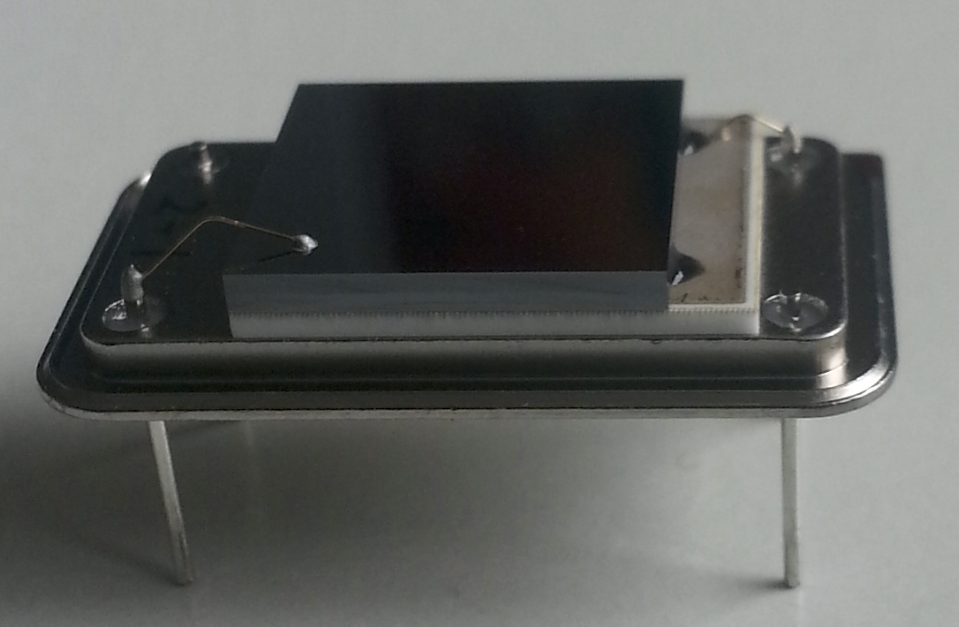
\includegraphics[width=0.44\textwidth]{figures/CdTeSensor.png} 
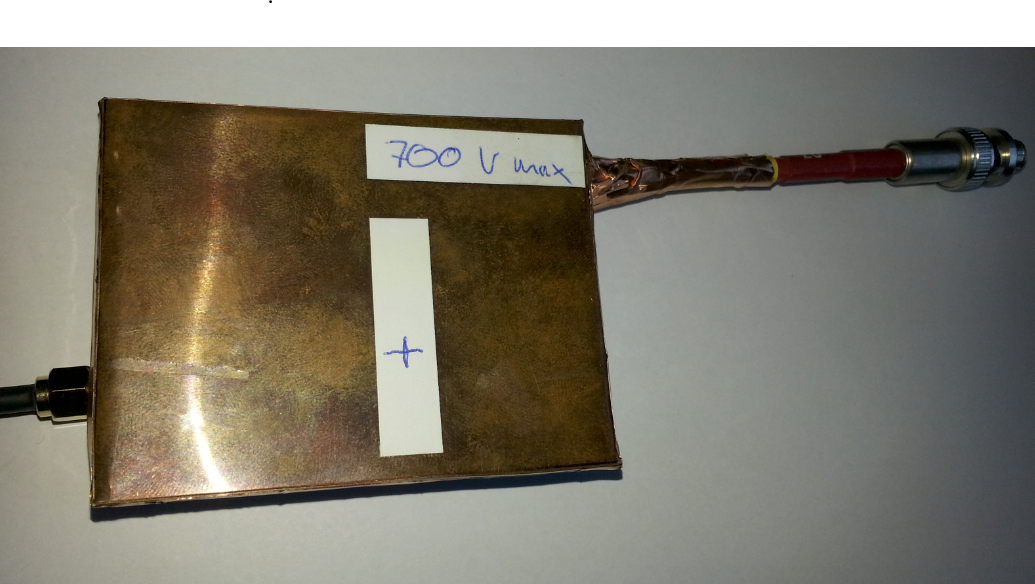
\includegraphics[width=0.55\textwidth]{figures/CdTeSensorBox.png} 
\caption{Left: CdTe sensor used for the measurements. The sensor is a Schottky type diode with a transverse size 
of $1$~$\mathrm{cm}^{2}$ and a thickness of $1$~mm. The baseplate is biased at $700$~V. 
On the front-left corner of the sensor, the wire bond connection
to the metalized top layer of the sensor can be seen. On the back-right corner,
the wirebond connection to the baseplate can be seen. 
Right: A photograph of the copper box enclosing the CdTe sensor. } 
\label{fig:CdTeSensor} 
\end{figure} 
%
The electrical circuit shown in Fig.~\ref{fig:cdtecircuit} was used to connect to the sensor to the bias 
voltage with a standard high voltage cable and the readout electronics using a SMA cable with a feed 
through penetrating the copper box.

%
\begin{figure}[htbp] 
\centering
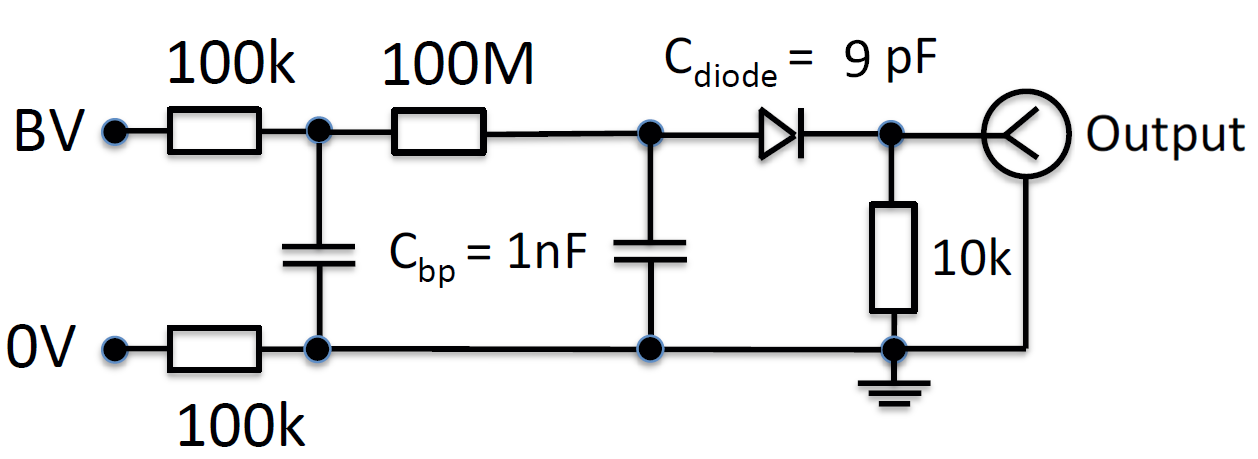
\includegraphics[width=0.49\textwidth]{figures/circuit_CdTe.png} 
\caption{Schematic diagram of the circuit used to polarize and read out the 
CdTe sensor. The circuit and the sensor are enclosed inside a copper box. }
\label{fig:cdtecircuit} 
\end{figure} 
%
